\documentclass[11pt,a4paper]{article}
\usepackage[margin=25mm]{geometry}
\usepackage[T1]{fontenc}
\usepackage{lmodern}
\usepackage{amsmath,amssymb}
\usepackage{booktabs,tabularx,array}
\newcolumntype{Y}{>{\raggedright\arraybackslash}X}
\usepackage{tikz}
\usetikzlibrary{arrows.meta,positioning,shapes.geometric,fit}
\usepackage{listings}
\usepackage[hidelinks]{hyperref}
\usepackage{xcolor}

\lstset{basicstyle=\ttfamily\small,columns=fullflexible,frame=single,framerule=0.3pt}
\newcommand{\code}[1]{\texttt{#1}}

\title{\textbf{eikos-search}\\[2pt]\large Specification}
\author{}
\date{}

\begin{document}
\maketitle

\section{Objective}

eikos-search is a web search tool that answers a question with \emph{the exact sentence of an existing article} that
states the answer. It uses Eikos, the open counterpart of the Jev ``System-1'' typed-decision model, to choose that
sentence.
\begin{itemize}
  \item It differs from a generative LLM because it \textbf{never writes an answer}. Every character shown to the user
        is a slice of a fetched article.
  \item It differs from an ordinary search engine because it shows \textbf{one exact phrase in the most relevant
        article} instead of a list of links.
\end{itemize}

\begin{table}[htbp]
\centering
\caption{The three ways to answer a question. eikos-search keeps the verifiability of search and the directness of
an LLM, and gives up the ability to answer what no article states.}
\label{tab:position}
\begin{tabularx}{\linewidth}{@{}p{30mm}YYY@{}}
\toprule
 & Generative LLM & Web search engine & \textbf{eikos-search} \\
\midrule
Output & newly generated text & ranked list of links & one verbatim sentence + its source \\
Can hallucinate & yes & no & no (output $\subseteq$ article text) \\
Reading left to the user & none & open and read the pages & none \\
When no source states the answer & answers anyway & shows links anyway & abstains \\
\bottomrule
\end{tabularx}
\end{table}

\section{Why Eikos}

Eikos (\href{https://github.com/caiovicentino/eikos}{github.com/caiovicentino/eikos}) does not generate text. Given a
\emph{state} (evidence), a \emph{criterion} and a list of options with descriptions, it reads one letter logit per
option in a single forward pass and returns calibrated probabilities over the options. Options are labelled
\code{A..Z, AA, AB, \dots} (up to 588 one-token labels). Above the model's one-pass limit $M$ (100 for the 4B models,
160 for the 27B models), a tournament runs: the options are split into blocks, and the best of each block go on to the
next round.

Here the options are the candidate sentences themselves. An Eikos choice is therefore a sentence that exists verbatim
in a source article, and the model has no way to produce anything else.

\section{Pipeline}

\begin{figure}[htbp]
\centering
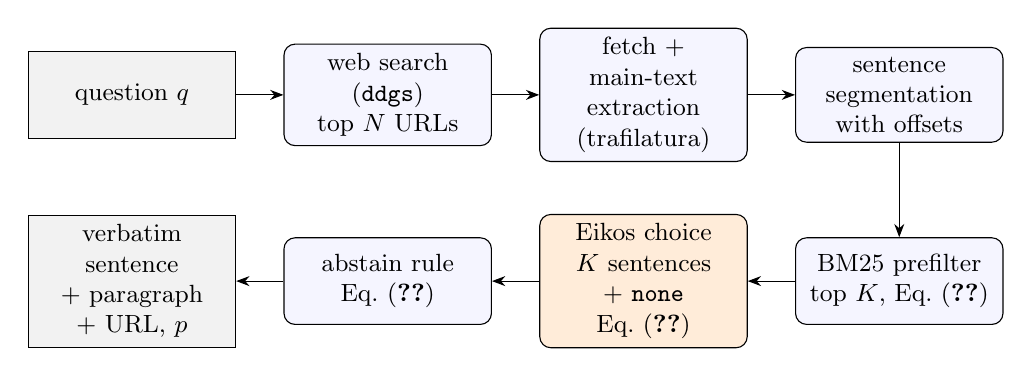
\begin{tikzpicture}[node distance=5mm and 6mm,
  box/.style={draw,rounded corners,align=center,minimum height=11mm,text width=24mm,font=\small,fill=blue!4},
  model/.style={box,fill=orange!15},
  io/.style={box,fill=gray!10,rounded corners=0},
  >={Stealth}]
\node[io]   (q)  {question $q$};
\node[box,  right=of q]  (s)  {web search\\(\code{ddgs})\\top $N$ URLs};
\node[box,  right=of s]  (f)  {fetch + main-text\\extraction\\(trafilatura)};
\node[box,  right=of f]  (g)  {sentence\\segmentation\\with offsets};
\node[box,  below=12mm of g] (b) {BM25 prefilter\\top $K$, Eq.~\eqref{eq:bm25}};
\node[model,left=of b]  (e)  {Eikos choice\\$K$ sentences + \code{none}\\Eq.~\eqref{eq:softmax}};
\node[box,  left=of e]  (a)  {abstain rule\\Eq.~\eqref{eq:abstain}};
\node[io,   left=of a]  (o)  {verbatim sentence\\+ paragraph\\+ URL, $p$};
\draw[->] (q)--(s); \draw[->] (s)--(f); \draw[->] (f)--(g); \draw[->] (g)--(b);
\draw[->] (b)--(e); \draw[->] (e)--(a); \draw[->] (a)--(o);
\end{tikzpicture}
\caption{Data flow for one question. Only the orange stage runs a neural network, and its output is an index into
sentences that already exist.}
\label{fig:pipeline}
\end{figure}

\begin{enumerate}
  \item \textbf{Search.} The configured backend returns up to $N$ hits (\code{search.max\_results}). Only
        \code{http(s)} URLs are kept, and duplicates are removed.
  \item \textbf{Fetch and extract.} Pages are fetched in parallel with a timeout (\code{search.timeout\_s}).
        Each request and each redirect hop (at most 5) goes only to a host whose every resolved address is public, and the connection is pinned to that address. Search results are third-party input, so this stops a result from reaching localhost or the LAN. Trafilatura extracts the main text and drops comments and tables. A page that fails to fetch or extract is
        skipped and logged.
  \item \textbf{Segment.} The text is split into paragraphs at newlines, and each paragraph is split into sentences:
        after \code{.!?} followed by whitespace (a citation marker such as \code{[20]} in between is skipped), or after the CJK full stops (U+3002, U+FF01, U+FF1F). Each sentence is stored as the
        offsets $(s,e)$ into the article text, with its paragraph's offsets. Sentences outside
        $[\code{min\_chars}, \code{max\_chars}]$ are dropped.
  \item \textbf{Prefilter.} Identical sentences are merged. If more than $K$ remain (\code{rank.prefilter\_k}),
        BM25~\eqref{eq:bm25} keeps the top $K$, in document order. This bounds the Eikos prompt length.
  \item \textbf{Choose.} One Eikos \code{choice} decision is made over the $K$ sentences plus a \code{none} option.
  \item \textbf{Answer or abstain.} The abstain rule~\eqref{eq:abstain} decides whether a sentence is shown.
\end{enumerate}

\section{Scoring}

\paragraph{BM25 prefilter.} The question $q$ and every sentence $d$ are tokenized. Latin-script text is split into
lower-cased words, and runs of CJK characters into character bigrams, because CJK text has no spaces. With $f(t,d)$ the
term frequency, $|d|$ the length of $d$ and $\overline{|d|}$ the mean length,
\begin{equation}
  \mathrm{BM25}(q,d)=\sum_{t\in q}\mathrm{IDF}(t)\,
  \frac{f(t,d)\,(k_1+1)}{f(t,d)+k_1\left(1-b+b\,|d|/\overline{|d|}\right)},\qquad k_1=1.5,\ b=0.75.
  \label{eq:bm25}
\end{equation}

\paragraph{Eikos choice.} The options are $o_1,\dots,o_K$ (the sentences, each described as ``\textit{sentence}
(from: \textit{article title})'') and $o_{K+1}=\code{none}$. The evidence is ``Question: $q$''. The criterion asks
which passage directly and explicitly states the answer, and to choose \code{none} if no passage does. Eikos reads
the logit $z_i$ of option $i$'s letter and returns
\begin{equation}
  p_i=\frac{\exp(z_i/T)}{\sum_{j=1}^{K+1}\exp(z_j/T)},\qquad
  T=\exp\!\bigl(b_0+\mathbf w^{\top}\mathbf f\bigr),
  \label{eq:softmax}
\end{equation}
where $\mathbf f=(\log n_{\text{tok}}-6.5,\ \log(K{+}1)-1.2,\ 0,\ 0)$ and $(b_0,\mathbf w)$ come from the model's
shipped \code{calib.json}. These are the upstream calibration features, unchanged.

\paragraph{Abstain rule.} From~\eqref{eq:softmax}, the probability that \emph{some} candidate states the answer
is the mass outside \code{none},
\begin{equation}
  p_{\text{ans}}=\sum_{i=1}^{K}p_i=1-p_{K+1}.
  \label{eq:answered}
\end{equation}
Let $i^\ast=\arg\max_{1\le i\le K+1}p_i$, and let $\tau$ be \code{rank.abstain\_threshold}. Using \eqref{eq:softmax}
and \eqref{eq:answered}, the shown answer is
\begin{equation}
  \text{answer}=
  \begin{cases}
    o_{i^\ast} & \text{if } i^\ast\le K \text{ and } p_{\text{ans}}\ge\tau,\\
    \text{``no article states this exactly''} & \text{otherwise.}
  \end{cases}
  \label{eq:abstain}
\end{equation}
The rule thresholds $p_{\text{ans}}$ and not $p_{i^\ast}$, because articles often repeat a fact. Several correct
sentences then share the mass, so each one's own $p_i$ is small even when the answer is certain
(Table~\ref{tab:abstain}). The condition $i^\ast\le K$ abstains when \code{none} beats every single sentence.

\begin{table}[htbp]
\centering
\caption{Measured with Eikos-4B (bf16), $K{=}64$ plus \code{none}. A threshold on the top sentence's $p_{i^\ast}$
(the boiling-point row) would wrongly abstain. Rule~\eqref{eq:abstain} gets all three right.}
\label{tab:abstain}
\begin{tabularx}{\linewidth}{@{}p{48mm}rrY@{}}
\toprule
Question & $p_{i^\ast}$ & $p_{K+1}$ (\code{none}) & Result of \eqref{eq:abstain}, $\tau=0.5$ \\
\midrule
What is the boiling point of water at sea level? & 0.137 & 0.001 & answer (5 correct sentences share $\approx$0.5) \\
What year did Japan join the United Nations? & 0.687 & 0.000 & answer (``\dots 18 December 1956.'') \\
Who first rode a purple giraffe across the Pacific? & 0.469 & 0.469 & abstain ($i^\ast=\code{none}$) \\
\bottomrule
\end{tabularx}
\end{table}

\section{Data model}

\begin{table}[htbp]
\centering
\caption{Records passed between stages. Every text a user sees is derived from \code{Article.text} by slicing.}
\begin{tabularx}{\linewidth}{lY}
\toprule
Record & Fields \\
\midrule
\code{SearchHit} & \code{title}, \code{url}, \code{snippet} \\
\code{Article}   & \code{title}, \code{url}, \code{text} (extracted main text) \\
\code{Passage}   & \code{article}, \code{start}, \code{end}, \code{para\_start}, \code{para\_end};\;
                   \code{text}$\,=\,$\code{article.text[start:end]} \\
\code{Answer}    & \code{question}, \code{found}, \code{probability} ($p_{i^\ast}$), \code{answered} ($p_{\text{ans}}$), \code{text}, \code{paragraph},
                   \code{offset\_in\_paragraph}, \code{title}, \code{url}, \code{articles}, \code{candidates},
                   \code{seconds} \\
\bottomrule
\end{tabularx}
\end{table}

\noindent\textbf{Invariant.} For every answer shown,
\code{article.text[start:end]} \code{==} \code{answer.text}. The pipeline asserts it, and the tests check it for every segmented
sentence.

\section{Configuration}

All settings live in \code{config/config.yaml}. The config path is the program's only argument. Unknown keys are
rejected, and a section that omits keys prints which defaults it uses.

\begin{table}[htbp]
\centering
\caption{Configuration keys.}
\label{tab:config}
\begin{tabularx}{\linewidth}{llY}
\toprule
Key & Default & Meaning \\
\midrule
\code{model.size}        & \code{4b}  & Eikos size: \code{4b} or \code{27b} \\
\code{model.precision}   & \code{bf16} & \code{bf16}, \code{fp8} or \code{int4} \\
\code{model.backend}     & \code{transformers} & inference runtime, not a model: \code{transformers} (Hugging Face Transformers library, in-process) or \code{vllm} (vLLM inference server, separate process) \\
\code{model.device}      & \code{cuda} & torch device for \code{transformers} \\
\code{model.max\_tokens} & 12000 & longest prompt accepted \\
\code{model.vllm\_url}   & \code{null} & URL of \code{scripts/serve\_vllm.sh} when \code{backend=vllm} \\
\code{search.backend}    & \code{ddgs} & search backend (DuckDuckGo; no API key) \\
\code{search.max\_results} & 8 & $N$, articles fetched per question \\
\code{search.region}     & \code{us-en} & ddgs region \\
\code{search.engines}    & \code{bing, yahoo, duckduckgo} & engines queried by ddgs \\
\code{search.timeout\_s} & 10 & per-page fetch timeout (s) \\
\code{extract.min\_chars}, \code{max\_chars} & 40, 600 & sentence length bounds \\
\code{rank.prefilter\_k} & 64 & $K$ in \eqref{eq:bm25}, \eqref{eq:softmax} \\
\code{rank.abstain\_threshold} & 0.5 & $\tau$ in \eqref{eq:abstain} \\
\code{server.host}, \code{port} & \code{127.0.0.1}, 8000 & web UI address \\
\bottomrule
\end{tabularx}
\end{table}

\subsection{Model registry}

The pair (\code{model.size}, \code{model.precision}) is the single switch for the model. The registry in
\code{eikos\_search/models.py} maps it to a checkpoint (Table~\ref{tab:models}). Every component that loads weights,
the tokenizer or the calibration reads that one resolved build. A combination not in the registry is an error, never a
silent fallback. Every run prints the build it loaded, e.g.\ \code{model: Eikos-4B (4b, bf16) via transformers on
cuda}.

\begin{table}[htbp]
\centering
\caption{Eikos builds. The fp8/int4 builds are compressed-tensors checkpoints, which the upstream in-process loader
does not read, so they require \code{backend: vllm}. 27B in bf16 needs an 80\,GB-class GPU.}
\label{tab:models}
\begin{tabular}{llllr}
\toprule
size & precision & Hugging Face repo & backends & weights (GB) \\
\midrule
4b  & bf16 & \code{caiovicentino1/Eikos-4B}       & transformers, vllm & 9.3 \\
4b  & fp8  & \code{caiovicentino1/Eikos-4B-FP8}   & vllm & 5.8 \\
4b  & int4 & \code{caiovicentino1/Eikos-4B-INT4}  & vllm & 4.0 \\
27b & bf16 & \code{caiovicentino1/Eikos-27B}      & transformers, vllm & 55.6 \\
27b & fp8  & \code{caiovicentino1/Eikos-27B-FP8}  & vllm & 31.2 \\
27b & int4 & \code{caiovicentino1/Eikos-27B-INT4} & vllm & 19.4 \\
\bottomrule
\end{tabular}
\end{table}

The \code{decision\_config.json} shipped with the model supplies the prompt style (set before \code{decision\_core} is
imported), the calibration file and the one-pass limit $M$.

\subsection{Search backends}

\code{search.backend} names one entry of the registry in \code{eikos\_search/search.py}. The only entry is
\code{ddgs}. Adding a backend means adding one function that returns \code{SearchHit} records.

\section{Interfaces}

\begin{lstlisting}
uv run eikos-search config/config.yaml          # web UI at http://127.0.0.1:8000
uv run eikos-search config/config.yaml --repl   # ask in the terminal
\end{lstlisting}

\paragraph{HTTP API.} \code{GET /} serves the page. \code{POST /api/answer} takes \code{\{"question": "..."\}} and
returns the \code{Answer} record as JSON. An empty question returns 422.

\paragraph{Web page.} The page shows the sentence as a quotation, then its paragraph with the sentence highlighted, then
the article title and link, then $p_{i^\ast}$, $p_{\text{ans}}$, the counts and the latency. All article text is inserted as text nodes, never as
HTML, and the link is rendered only for \code{http}/\code{https} URLs.

\section{Dependencies}

Eikos is vendored as a git submodule at \code{third\_party/eikos}, pinned to an upstream commit. The project calls its
internals (\code{letter\_adapter.LetterAdapter}, \code{decision\_core}), so its version determines the probabilities in
\eqref{eq:softmax}. Clone with \code{git clone --recursive}. Other dependencies are managed by \code{uv}.

\section{Non-goals}

\begin{itemize}
  \item Generating, paraphrasing or summarising answers.
  \item Answers that need to combine several sentences, or multi-step reasoning (Eikos does not reason across steps).
  \item Content that is not in the extracted main text: tables, images, PDFs.
  \item Guaranteeing that the source is true. The tool guarantees only that the source says it.
\end{itemize}

\end{document}
